\documentclass[titlepage,11pt]{article}
\usepackage{amsmath}
\usepackage{tikz}

\begin{document}

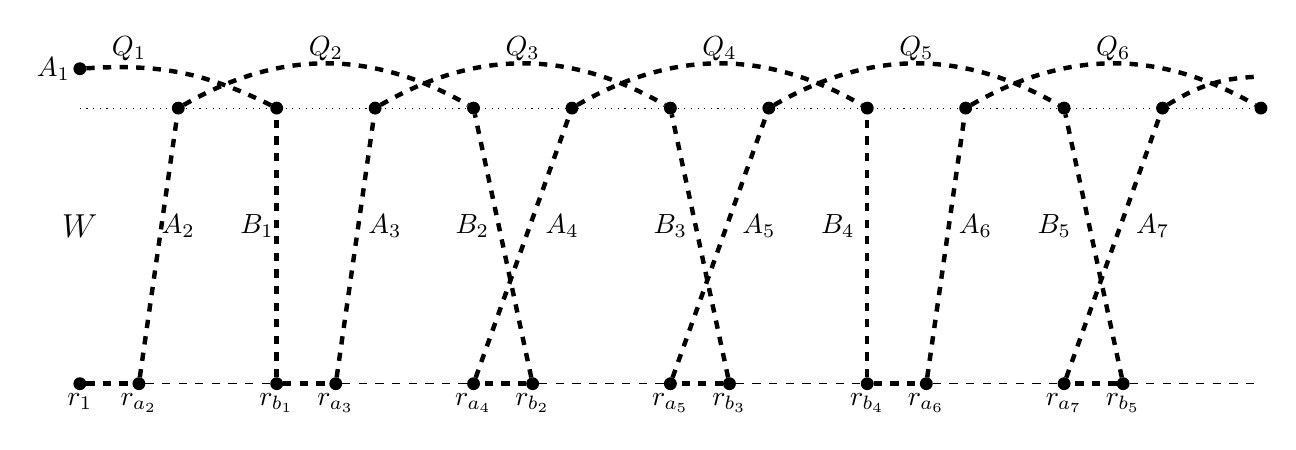
\begin{tikzpicture}[scale=1/2,auto=left]

\def\c{7}
\draw[dotted]  (0,\c)--(30,\c);
\tikzstyle{every node}=[inner sep=1.5pt, fill=black,circle,draw]
\node (r1) at (0,0) {};
\node (ra2) at (1.5,0) {};
\node (rb1) at (5,0) {};
\node (ra3) at (6.5,0) {};
\node (ra4) at (10,0) {};
\node (rb2) at (11.5,0) {};
\node (ra5) at (15,0) {};
\node (rb3) at (16.5,0) {};
\node (rb4) at (20,0) {};
\node (ra6) at (21.5,0) {};
\node (ra7) at (25,0) {};
\node (rb5) at (26.5,0) {};


\node (a1) at (0,\c+1) {};
\node (a2) at (2.5,\c) {};
\node (b1) at (5,\c) {};
\node (a3) at (7.5,\c) {};
\node (b2) at (10,\c) {};
\node (a4) at (12.5,\c) {};
\node (b3) at (15,\c) {};
\node (a5) at (17.5,\c) {};
\node (b4) at (20,\c) {};
\node (a6) at (22.5,\c) {};
\node (b5) at (25,\c) {};
\node (a7) at (27.5,\c) {};
\node (b6) at (30,\c) {};


\tikzstyle{every node}=[]
\draw[below] (r1) node []           {$r_1$};
\draw[below] (ra2) node []           {$r_{a_2}$};
\draw[below] (rb1) node []           {$r_{b_1}$};
\draw[below] (ra3) node []           {$r_{a_3}$};
\draw[below] (ra4) node []           {$r_{a_4}$};
\draw[below] (rb2) node []           {$r_{b_2}$};
\draw[below] (ra5) node []           {$r_{a_5}$};
\draw[below] (rb3) node []           {$r_{b_3}$};
\draw[below] (rb4) node []           {$r_{b_4}$};
\draw[below] (ra6) node []           {$r_{a_6}$};
\draw[below] (ra7) node []           {$r_{a_7}$};
\draw[below] (rb5) node []           {$r_{b_5}$};


\def\d{4}
\draw (2.5,\d) node [] {$A_2$};
\draw (4.5,\d) node [] {$B_1$};
\draw (7.75,\d) node [] {$A_3$};
\draw (9.97,\d) node [] {$B_2$};
\draw (12.25,\d) node [] {$A_4$};
\draw (15,\d) node [] {$B_3$};
\draw (17.25,\d) node [] {$A_5$};
\draw (19.25,\d) node [] {$B_4$};
\draw (22.75,\d) node [] {$A_6$};
\draw (24.75,\d) node [] {$B_5$};
\draw (27.25,\d) node [] {$A_7$};
\draw (0,\d) node [] {\large $W$};

\draw[left] (a1) node []           {$A_1$};
\draw (1.25,\c+1.5) node []           {$Q_1$};
\draw (6.25,\c+1.5) node []           {$Q_2$};
\draw (11.25,\c+1.5) node []           {$Q_3$};
\draw (16.25,\c+1.5) node []           {$Q_4$};
\draw (21.25,\c+1.5) node []           {$Q_5$};
\draw (26.25,\c+1.5) node []           {$Q_6$};




\draw[dashed, ultra thick] (ra2)--(a2);
\draw[dashed, ultra thick] (ra3)--(a3);
\draw[dashed, ultra thick] (ra4)--(a4);
\draw[dashed, ultra thick] (ra5)--(a5);
\draw[dashed, ultra thick] (ra6)--(a6);
\draw[dashed, ultra thick] (ra7)--(a7);

\draw[dashed, ultra thick] (rb1)--(b1);
\draw[dashed, ultra thick] (rb2)--(b2);
\draw[dashed, ultra thick] (rb3)--(b3);
\draw[dashed, ultra thick] (rb4)--(b4);
\draw[dashed, ultra thick] (rb5)--(b5);

\draw[dashed, ultra thick] (a2) to [bend left = 30] (b2);
\draw[dashed, ultra thick] (a3) to [bend left = 30] (b3);
\draw[dashed, ultra thick] (a4) to [bend left = 30] (b4);
\draw[dashed, ultra thick] (a5) to [bend left = 30] (b5);
\draw[dashed, ultra thick] (a6) to [bend left = 30] (b6);
\draw[dashed, ultra thick] (b1) to [bend right = 15] (a1);
\draw[dashed, ultra thick] (a7) to [bend left = 15] (30,\c+.8);

\draw[dashed, ultra thick] (r1) to (ra2);
\draw[dashed, ultra thick] (rb1) to (ra3);
\draw[dashed, ultra thick] (rb2) to (ra4);
\draw[dashed, ultra thick] (rb3) to (ra5);
\draw[dashed, ultra thick] (rb4) to (ra6);
\draw[dashed, ultra thick] (rb5) to (ra7);
\draw[dashed] (ra2) to (rb1);
\draw[dashed] (ra3) to (ra4);
\draw[dashed] (rb2) to (ra5);
\draw[dashed] (rb3) to (rb4);
\draw[dashed] (ra6) to (ra7);
\draw[dashed] (rb5) to (30,0);

\end{tikzpicture}

\end{document}